\chapter{RespVis Modules}
\label{chap:Modules}

The source code of RespVis is structured into modules written in the
ES module format. Currently, all individual modules are combined into
a single, monolithic library bundle during the build process, but this
will be changed in the future so that visualization authors can import
only the modules they need. The reason for this is that most authors
will likely require only a subset of all the features included in the
library, and it would unnecessarily increase the size of their bundles
to import them all. A good example of this is D3, which also separates
its extensive collection of functionality into different modules which
can be successively added to a project as the need arises.

At the time of writing, the RespVis library comprises five modules:
\modname{Core Module}, \modname{Legend Module}, \modname{Tooltip
  Module}, \modname{Bar Module}, and \modname{Point Module}, each
containing various submodules grouped by thematic similarity. The
\modname{Core Module} holds the core functionality of the library
which all other modules depend on, including the \smodname{Layouter}
and \smodname{Axis Components}, \smodname{Chart} and \smodname{Chart
  Window} base functionality, and various utility functions and
types. The \modname{Legend Module} contains the implementation of a
\smodname{Legend Component} to identify discrete data by rendering a
legend of distinct values as labeled symbols. The \modname{Tooltip
  Module} holds functions to control the display, placement, and
content of \smodname{Tooltips}, as well as utility functions to
simplify the configuration and initialization of \smodname{Tooltips}
on \smodname{Series Components}. The \modname{Bar Module}
distinguishes between \smodname{Single-Series}, \smodname{Grouped},
and \smodname{Stacked Bars} and includes various low-level and
high-level components to render each of those types. Similarly, the
\modname{Point Module} contains low-level and high-level components to
visualize \smodname{Point Charts}. All of the different modules and
the dependencies between them are shown in Figure~\ref{fig:Modules}.


\begin{figure}[tp]
\centering
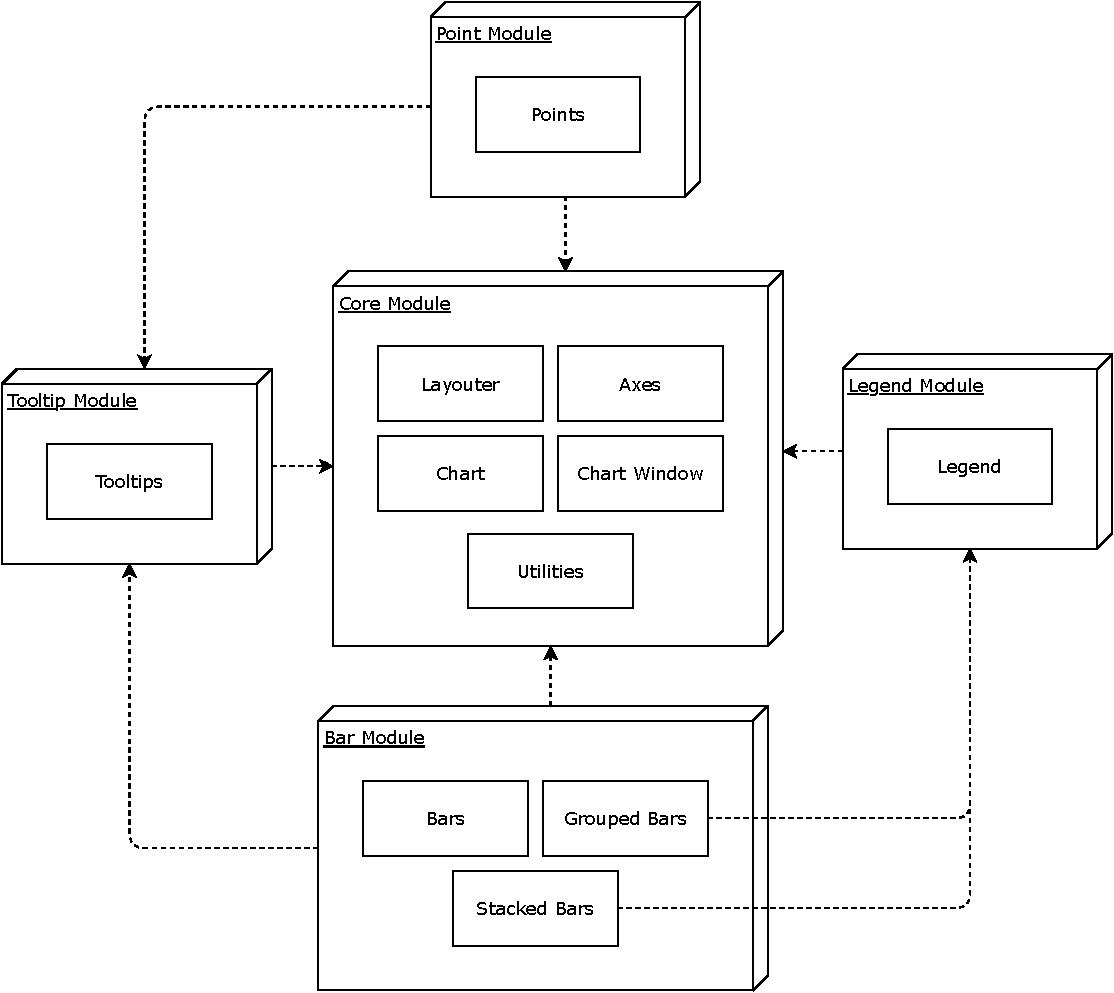
\includegraphics[keepaspectratio,width=\linewidth,height=\fullh]
{diagrams/respvis-modules.pdf}
\caption[Modules of RespVis]{
The five modules of the RespVis library and their submodules. The
directional arrows indicate dependencies between modules.
\imgcredit{Image created by the author of this thesis using
  \href{https://diagrams.net/}{diagrams.net}.}
}
\label{fig:Modules}
\end{figure}







\section{Core Module}

The implementation of the Core Module is located in the
\code{src/lib/core/} directory of the project and contains the
necessary core functionality of the library. It forms the base on
which all other modules depend and includes various utility functions,
the Layouter, Axes, Chart base functionality, and Chart Window base
functionality.  RespVis heavily relies on utility functions to reuse
recurring operations, and the Core Module contains utilities which
simplify the handling of arrays, elements, Selections, texts,
positions, sizes, rectangles, circles, and paths. The Layouter is a
custom component which enables the layout of SVG elements with CSS.
Axis Components have been included in the Core Module because they are
important components which occur in nearly all visualizations.  Lastly,
the Core Module offers base functionality for Charts and Chart
Windows to simplify the creation of more specialized Chart and Chart
Window Components.


\subsection{Utilities}

The utilities provided by RespVis are split into multiple submodules
placed in the \code{utilities/} directory of the Core Module. These
modules include types and functions to perform array, element,
selection, and text operations, as well as modules to simplify
geometric operations with positions, sizes, rectangles, circles, and
paths.  Utility functions are grouped into submodules by the type of
entity on which they operate, which is is also reflected in the
utility function names.  The names of utility functions follow the
top-down naming convention described in
Section~\ref{sec:NamingConventions}, which means that the names all
begin with the type of entity with which the function is associated.

Array utilities can be found in the Array Utilities Module in the file
\code{utilities/array.ts}.  The \code{Array} class in the JavaScript
base implementation already offers a wide variety of convenient
methods to work with arrays.  These methods form a solid foundation to
handle a broad range of situations, but not everything is covered, and
some things require manual implementations, which is why the RespVis
library offers additional functions to simplify commonly encountered
tasks.  The \code{arrayEquals} function is used to verify the equality
of two arrays and also works with arbitrary levels of nesting. Array
type guard functions are used to determine at runtime whether or not a
variable is an array. The function \code{arrayIs} evaluates to true if
the passed parameter is any kind of array, and \code{arrayIs2D}
evaluates to true if the passed parameter is a two-dimensional array.
The \code{arrayIs} function is merely an alias for the
\code{Array.isArray} method and has been added to provide a consistent
counterpart to the \code{arrayIs2D} type guard function. The last
function in the Array Utility Module is the \code{arrayPartition}
function, which receives an array and a partition size as parameters
and returns a partitioned version of the input array with each chunk
containing the number of items specified by the partition size
parameter.


The Element Utility Module located at \code{utilities/elements.ts} in
the Core Module contains functions and constants related to elements
in a document.  The \code{elementRelativeBounds} function is used to
calculate the bounding box of an element relative to the bounding box
of its parent in viewport coordinates.  Internally, it uses the
\code{getBoundingClientRect} function, which returns the actual
bounding box of an element in viewport coordinates and, as opposed to
other ways of accessing this information, this function also takes
transformations into account.  Every element has a set of CSS styles
applied to them, and the \code{Window.getComputedStyle} method is used
to query the active styles of elements. The style declaration object
returned by this method contains all possible CSS properties and their
values, regardless of whether or not they are set to default values.
Sometimes this behavior may be desired, but in this library, the
computed style is mainly used for the preparation of a downloadable
SVG document to transform styling information set in CSS to attributes
on the individual elements. If every possible CSS property on every
element would be mapped to an attribute, the resulting SVG document
would be unnecessarily bloated and hard-to-read, because only those
properties that are not set to their default values actually have an
effect. For this reason, the
\code{elementComputedStyleWithoutDefaults} function has been
implemented to calculate the computed style of an element and remove
all default-valued properties from the returned style declaration
object.  This is implemented by adding a \elname{<style-dummy>} element
as a sibling of the element of interest, getting the computed styles
of both elements, and calculating the difference between them.  To
accelerate these calculations, the
\code{elementComputedStyleWithoutDefaults} function accepts an array
of property names as its second parameter and will only consider the
properties listed in this array.  The constant
\code{elementSVGPresentationAttrs} array contains the names of all SVG
presentation attributes listed in the SVG 1.1 specification
\parencite{SVG11}.  As soon as support for SVG 2 \parencite{SVG2} by
most major browsers has reached maturity, this array will be extended
to include any newly added presentation attributes.  Since only these
SVG attributes can be styled via CSS, only CSS properties representing
presentation attributes have to be considered when preparing
downloadable SVG documents.

Selection utilities are implemented in the Selection Utilities Module
in file \code{utilities/selection.ts} and include typing improvements
for the D3 \code{Selection}, \code{Transition}, and
\code{SelectionOrTransition} interfaces and type guards to distinguish
between them.  The \code{Selection}, \code{Transition}, and
\code{SelectionOrTransition} interfaces allow the specification of
four type variables: the type of elements contained in the Selection
or Transition, the type of data bound to those elements, the type of
the parents of those elements, and the type of data bound to those
parents.  In most cases, the type variables related to parent elements
do not influence the logic of code using these interfaces and could be
omitted to keep it more concise.  For this reason, these interfaces
have been reexported with default types set on all of the type
variables, which means that whenever type variables need to be
manually specified, only those that need to be set to specific types
need to be explicitly stated.  Further typing improvements have been
made to the \code{attr} and \code{dispatch} methods of the
\code{Selection} interface.  The D3 type declarations of the
\code{Selection.attr} method do not include \code{null} as a possible
return value, which is wrong because this method will result in a
\code{null} value when reading an attribute that does not exist.  To
fix this inconsistency and catch potential bugs related to it during
compilation, the type declaration of the \code{Selection.attr} method
has been overwritten in the Selection Utility Module to include
\code{null} as a possible return value.  A less important but
convenient improvement has been made to the type declaration of the
\code{Selection.dispatch} method, which allows the dispatching of
custom events with certain parameters that control different aspects
of how this event is dispatched and the data bound to it.  In
practice, not all parameters need to be specified at every invocation
because the implementation of the \code{Selection.dispatch} method
will provide default values for all of them, but this is not reflected
in the type declaration of the function, which requires every
parameter to be set every time the function is called.  To fix this,
the Selection Utility Module provides a type declaration overwrite for
the \code{Selection.dispatch} function that wraps the type of the
parameters parameter into the \code{Partial} utility type.  Apart from
these typing improvements, this module also provides the
\code{isSelection} and \code{isTransition} type guard functions that
are used to distiguish between Selections and Transitions.


Utilities for dealing with \elname{<text>} elements can be found in the
Text Utilities Module in file \code{utilities/text.ts}, which contains
basic functionality to set specific \code{data-*} attributes to
specific values on \elname{<text>} elements. The Text Utility Module
holds functions that set \code{data-*} attributes controlling the
horizontal and vertical alignment of \elname{<text>} elements, as well
as their orientation.  Horizontal and vertical alignment is configured
using the \code{textAlignHorizontal} and \code{textAlignVertical}
functions, which respectively set the \code{data-align-h} and
\code{data-align-v} attribute on \elname{<text>} elements to the value
passed into either function as a string enum parameter of type
\code{HorizontalAlignment} or \code{VerticalAlignment}.  The
\code{HorizontalAlignment} enum represents the string values
\code{\"left\"}, \code{\"center\"} and \code{\"right\"}, while the
\code{VerticalAlignment} enum represents the values \code{\"top\"},
\code{\"center\"} and \code{\"bottom\"}.  The distinct
\code{data-align-h} and \code{data-align-v} attribute values are then
used in Selectors of various CSS rules to declare different values for
the \code{text-anchor} and \code{dominant-baseline} properties.  Text
orientation is set using the \code{textOrientation} function, which
sets the \code{data-orientation} attribute on \elname{<text>} elements
to the value specified via the \code{Orientation} string enum
parameter.  The \code{Orientation} enum represents the values
\code{\"horizontal\"} and \code{\"vertical\"}.  These
\code{data-orientation} attribute values are then used in CSS to set
the \code{text-anchor}, \code{dominant-baseline}, and \code{transform}
properties of \elname{<text>} elements, in order to rotate them
accordingly and position them correctly inside their bounding box
calculated by the Layouter.


The Core Module also contains utilities to simplify geometric
operations. One of these utility modules is the Position Utility
Module located in the \code{utilities/position.ts} file, which
contains the \code{Position} interface and various functions to
perform operations related to it. The \code{Position} interface
consists of the \code{x} and \code{y} number properties. Rounding
these properties is necessary to be able to correctly compare the
equality of two \code{Position} objects and to not render
unnecessarily long strings when transforming them into string
representations. This rounding is performed with the
\code{positionRound} function, which allows the specification of the
number of decimals the properties should be rounded to. Equality
comparision between two \code{Position} objects can be done with the
\code{positionEquals} function, which evaluates to \code{true} if all
properties of both \code{Position} objects are equal and \code{false}
if not.  The \code{positionToString} function can be used to transform
a \code{Position} object into its \code{\"x, y\"} string
representation, and its counterpart, the \code{positionFromString}
function, can be used to transform a correctly-formatted string into a
\code{Position} object.  A large part of RespVis consists of modifying
the attributes of elements.  Therefore, the \code{positionToAttrs}
function can be used to set the \code{x} and \code{y} attributes of
elements to the values of the \code{x} and \code{y} members of a
\code{Position} object, and similarly, the
\code{positionToTransformAttr} function can be used to set the
\code{transform} attribute of elements to a translation representing a
\code{Position} object.  The Position Utility Module also contains the
\code{positionFromAttrs} function, which can be used to create a
\code{Position} object from an element's \code{x} and \code{y}
attributes.

The Size Utility Module located in the \code{utilities/size.ts} file
in the Core Module is very similar to the Position Utility Module.  It
contains the \code{Size} interface, which consists of the \code{width}
and \code{height} number properties, the \code{sizeRound} function to
round the properties of a \code{Size} object to a certain number of
decimals, and the \code{sizeEquals} function to compare two
\code{Size} objects for equality.  Similar to the equivalent functions
in the Position Utility Module, the \code{sizeToString} and
\code{sizeFromString} functions can be used to convert between
\code{Size} objects and their string representations, and the
\code{sizeToAttrs} and \code{sizeFromAttrs} functions can be used to
convert between \code{Size} objects and \code{width} and \code{height}
attributes of elements.

Utilities for dealing with rectangles can be found in the Rectangle
Utility Module, which is located in the \code{utilities/rect.ts} file
of the Core Module.  This module contains the \code{Rect} interface,
which is the union of the \code{Position} and \code{Size} interfaces
and therefore describes an object with the \code{x}, \code{y},
\code{width}, and \code{height} number properties.  Similar to the
Position and Size Utility Modules, this module contains the
\code{rectRound} function to round \code{Rect} objects, the
\code{rectEquals} function to compare two of them for equality, the
\code{rectToString} and \code{rectFromString} functions to convert
between \code{Rect} objects and their string representations, and the
\code{rectToAttrs} and \code{rectFromAttrs} functions to convert
between objects and \code{x}, \code{y}, \code{width}, and
\code{height} attributes of elements.  Since the \code{Rect} interface
is a combination of the \code{Position} and \code{Size} interfaces,
most of the functions in this module internally use the functions
provided by the Position and Size Utility Modules.  The
\code{rectMinimized} function creates a minimized version of the
passed \code{Rect} object, which is infinitely small and positioned at
the original \code{Rect} object's center.  Minimized rectangles are
used in transitions that grow or shrink \elname{<rect>} elements from or
to their centers.  When declaring a stroke for SVG elements, it is
drawn exactly on the outline of an element's shape, which means that a
stroke will extend outside the original bounds of an element by half
the stroke width.  This can lead to unwanted artifacts like the stroke
of bars in a Bar Chart overlapping over the Chart's Axes.  To
counteract this, the \code{rectFitStroke} function is offered by the
Rect Utility Module to adjust the properties of \code{Rect} objects to
account for a specific stroke width around them.  Lastly, the
Rectangle Utility Module provides functions to calculate specific
positions inside rectangles. The most generic of these functions is
the \code{rectPosition} function, which enables the calculation of a
position inside a rectangle via a two-dimensional parameter which
expresses a position as the percentual width and height distance from a
rectangle's top-left corner. All other position-calculating rectangle
utility functions are simply shorthand functions that internally call
the \code{rectPosition} function.  The \code{rectCenter} function
returns a \code{Position} object representing the center position of a
\code{Rect} object.  The \code{rectLeft}, \code{rectRight},
\code{rectTop}, and \code{rectBottom} functions return \code{Position}
objects that represent the middle position of the corresponding edge
of a \code{Rect} object.  Similarly, The \code{rectTopLeft},
\code{rectTopRight}, \code{rectBottomRight}, \code{rectBottomLeft}
functions can be used to calculate the corner positions of a
rectangle.

The Circle Utility Module can be found in the
\code{utilities/circle.ts} file in the Core Module.  It contains the
\code{Circle} interface, which describes a circle object via a
\code{center} \code{Position} property and a \code{radius} number
property.  This module also contains equivalent functions to those
found in previously-mentioned utility modules: \code{circleRound},
\code{circleEquals}, \code{circleToString}, \code{circleFromString},
\code{circleToAttrs}, \code{circleFromAttrs}, \code{circleMinimized},
and \code{circleFitStroke}.  Furthermore, the \code{circlePosition}
function can be used to calculate positions inside a circle using an
angle that defines an offset direction and an offset distance from a
circle's center as a percentage of the circle's radius.  The Circle
Utility Module also contains functions to create circles from
rectangles, which are the \code{circleInsideRect} function to
calculate the largest circle that can fit inside of a rectangle and
the \code{circleOutsideRect} function to calculate the smallest circle
that encloses a rectangle.

The Path Utility Module is located in the \code{utilities/path.ts}
file in the Core Module and provides functions to simplify the
creation of path definitions that can be set as \code{d} attributes on
\elname{<path>} elements.  The \code{pathRect} function uses a
\code{Rect} object to create a rectangle path definition that can be
set on \elname{<path>} elements instead of using \elname{<rect>} elements.
Similarly, the \code{pathCircle} function uses a \code{Circle} element
to create a circle path definition that can be set on \elname{<path>}
elements instead of using a \elname{<circle>} elements. The reasons for
using \elname{<path>} elements rather than more descriptive shape
elements is that their shapes can be changed dynamically and it
is possible to smoothly transition between shapes by interpolating
their path definition strings.



\subsection{Layouter}
\label{sec:Layouter}

The Layouter is the most novel contribution of this work.  It is a
component which wraps around an SVG document and allows configuration
of the layout of elements in this document with CSS constructs like
Grid and Flexbox. Instead of implementing a custom layout algorithm,
the Layouter utilises the layout engine already built in to the
browser, which were summarized in Section~\ref{sec:BrowserEngines}.
Earlier proof of concept implementations used the FaberJS
\parencite{FaberJS} and Yoga \parencite{Yoga} layout engines to
compute layouts, but these implementations limited layouting to either
Grid or Flexbox-based constraints. Furthermore, the use of built-in
browser functionality in the current implementation leads to a reduced
bundle size and to visualization authors being able to use all the
layouting capabilities natively offered by browsers.

CSS has always been the foundation of responsive web design for
HTML-based websites because of its ability to adapt an element's
presentation and the possibility of defining different presentations
for different contexts via media queries. A large part of the
responsive power of CSS comes from its ability to change the
positioning and layout of elements. As already mentioned in previous
chapters, CSS can style certain aspects of SVG documents, but it is
not possible to use CSS layouting techniques to position SVG elements.
Even though there are already other visualization libraries such as
Chartist \parencite{Chartist} and Highcharts \parencite{Highcharts}
which allow the use of CSS to style visualizations, none of them offer
the possibility to modify the layout of visualizations via CSS, which
means that visualization authors have to learn and use custom APIs to
position elements, limiting the range of possible layouts to those
supported by the individual libraries.

The RespVis Layouter distinguishes between laid-out and non-laid-out
elements, since not every element in a visualization profits from
being laid out. The positions and sizes of laid-out elements are
calculated by the Layouter, whereas non-laid-out elements are ignored
during the layout process. Theoretically, the Layouter could be used
to position all visualization elements, since all that is necessary is
to determine a good mapping for each element that maps the rectangular
bounding box calculated by the Layouter to the desired SVG shape of
the element. However, the positioning of elements in a visualization
is constrained more strictly than element positioning in typical HTML
documents, because the content of a visualization is communicated
through visual features such as position, size, shape, and poximity of
elements rather than simply through text which can be positioned much
more freely. For this reason, many elements of a visualization must be
positioned at specific locations with specific dimensions, which means
there is very little profit in laying them out with an elaborate
layout algorithm. Instead, exactly-positioned elements like the
\elname{<rect>} elements of Bar Series and the \elname{<circle>} elements
of Point Series are usually positioned directly via their SVG
attributes.

The Layouter Module can be found in the \code{layouter.ts} file of the
Core Module. The main function of this module is the
\code{layouterCompute} function which implements the three-phased
layout process shown in Figure~\ref{fig:LayoutProcess}. The three
phases are:
\begin{enumerate}
\item Replication: The structure of the SVG document that shall be
  laid out is replicated with HTML \elname{<div>} elements, because
  only HTML elements can be affected by CSS-based positioning. These
  elements are referred to as \enquote{layout elements} and have the
  same classes and \code{data-*} attributes as the SVG elements they
  are replicating.

\item Layout: The replicated layout elements are affected by CSS rules
  to configure their positioning and are automatically laid out by
  browsers. If the selectors of CSS rules used to style SVG elements
  only select them using classes and \code{data-*} attributes, the
  layout of these elements can be directly configured in these rules,
  because the corresponding layout elements have the same classes and
  \code{data-*} attributes and these CSS rules will also be applied to
  them.

\item Synchronization: In this phase, the positions of layout elements
  are synchronized with their respective SVG elements. The calculated
  bounding boxes of layout elements are set as \code{bounds}
  attributes on SVG elements to make the boundary information
  available in subsequent renderings for the positioning of nested
  elements. In addition, the Layouter sets different default
  attributes on different types of SVG elements that aim to represent
  the boundaries of individual elements.
\end{enumerate}




\begin{figure}[tp]
\centering
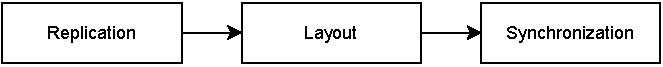
\includegraphics[keepaspectratio,width=\linewidth,height=\fullh]
{diagrams/respvis-layout-process.pdf}
\caption[Layout Process of the Layouter]{
The three phases of the layout process of the RespVis Layouter.
During the replication phase, the SVG document is replicated with HTML
\elname{<div>} elements. Afterwards, these HTML elements are laid out by
the browser in the layout phase, and the positions of the laid-out
HTML elements are applied to their respective SVG elements during the
synchronization phase.  \imgcredit{Image created by the author of this
  thesis using \href{https://diagrams.net/}{diagrams.net}.}
}
\label{fig:LayoutProcess}
\end{figure}



During the replication process, the structure of an SVG document is
replicated with HTML \elname{<div>} elements, which is implemented via a
hierarchical D3 data join, in which the original SVG elements are
bound as data objects to layout elements. The hierarchical data join
results in a counterpart in the hierarchy of layout elements for each
SVG element that should be affected by the Layouter.  Since not every
SVG element should be positioned via the Layouter, the Layouter must
be told which elements to ignore.  For this, the
\code{data-ignore-layout} and \code{data-ignore-layout-children}
attributes have been introduced.  Elements having the
\code{data-ignore-layout} attribute or which are children of elements
having the \code{data-ignore-layout-children} attribute will not be
replicated by the Layouter.

To configure the layout of such layout elements in CSS, it must be
possible to select them uniquely with a CSS selector. This selector
should be as similar as possible to the selector of their
corresponding SVG elements, to make it as easy as possible to
configure the CSS properties of layout elements. For this purpose, the
\code{class} attributes and all \code{data-*} attributes of SVG
elements are copied to their layout elements. In addition to the
classes of the replicated SVG element, the \code{layout} class is set
on all layout elements, which makes it possible to specifically select
an SVG element's layout element via the same selector extended by the
\code{layout} class. If CSS rules affecting SVG elements use only
classes and \code{data-*} attributes in their selectors, the
properties of corresponding layout elements can be directly configured
in the same rules, since these selectors will also match them. An
example of a replicated layout element tree of an SVG document can be
seen in Listing~\ref{list:LayouterStructure}. An example of CSS rules
to set various properties of SVG elements and their layout elements
can be seen in Listing~\ref{list:LayouterCSS}.


\begin{samepage}
\lstinputlisting[%
  float=tp,
  aboveskip=\floatsep,
  belowskip=\floatsep,
  xleftmargin=0cm,              % no extra margins for floats
  xrightmargin=0cm,             % no extra margins for floats
  %
  basicstyle=\footnotesize\ttfamily,
  frame=shadowbox,
  numbers=left,
  label=list:LayouterStructure,
  caption={[Replicated Layout Structure of an SVG Document]%
The replicated layout element structure of an SVG document. Every SVG
element has a corresponding layout element that has the same classes
and \code{data-*} attributes. In addition to the classes of the
original SVG element, every layout element also has the \code{layout}
class to allow specific targeting of layout elements via CSS
Selectors.
},
]{listings/layouter-structure.html}
\end{samepage}


\begin{samepage}
\lstinputlisting[%
  float=tp,
  aboveskip=\floatsep,
  belowskip=\floatsep,
  xleftmargin=0cm,              % no extra margins for floats
  xrightmargin=0cm,             % no extra margins for floats
  %
  basicstyle=\footnotesize\ttfamily,
  frame=shadowbox,
  numbers=left,
  label=list:LayouterCSS,
  caption={[CSS Rules to Style SVG]%
These CSS rules are used to configure the layout and style of an SVG
document that is being laid out by the Layouter. Since the selectors
of these CSS rules only use \code{class} and \code{data-*} attributes
to match elements, the same rule can be used to configure the
properties of an SVG element and its corresponding layout element.
The structure of the SVG document and its replicated layout elements
can be seen in Listing~\ref{list:LayouterStructure}.
},
]{listings/layouter-css.css}
\end{samepage}


The size of dynamically-sized elements depends on the size of their
content, and since layout elements exist separately from their SVG
elements and can not access their content, a manual solution had to be
implemented to set the size of layout elements to the content size of
their SVG elements when required. \elname{<text>} elements are a good
example of dynamically-sized elements, because their size is rarely
explicitly declared and usually depends on the size of their textual
content. The custom \code{--fit-width} and \code{--fit-height} CSS
properties were introduced to activate the manual copying of
dimensions from SVG elements to their layout elements. These boolean
properties can be set in CSS rules and are checked during the
replication phase via the \code{window.getComputedStyle} method. If at
least one of these properties is set to \code{true}, the dimensions of
the SVG element are calculated with the
\code{Element.getBoundingClientRect} method are set as \code{width} or
\code{height} properties in the \code{style} attribute on the
corresponding layout element. This way, layout elements will have the
same sizes as their SVG elements and can be properly used in the
calculation of the overall layout.

Layout elements are positioned according to the layout information
specified in CSS rules during the layout phase. Since layout elements
are merely \elname{<div>} elements which have been styled via CSS rules,
the browser can position them automatically via its integrated layout
engine, which happens immediately after they have been created or
updated in the replication phase.  After the layout phase, the final
bounding boxes of layout elements can be calculated and used for
further operations.

In the synchronization phase of the layout process, the Layouter
calculates the bounding boxes of all layout elements and sets this
boundary information as attributes on the corresponding SVG elements.
Bounding boxes of layout elements are calculated relative to their
parent elements using the \code{elementRelativeBounds} utility
function, converted to their string representations via the
\code{rectToString} utility function, and set as \code{bounds}
attributes on corresponding SVG elements.  These \code{bounds}
attributes can then be deserialized to \code{Rect} objects whenever
the bounding boxes of SVG elements are needed for calculations in
subsequent renderings. In addition to setting \code{bounds}
attributes, the Layouter also sets specific default attributes on
different types of SVG elements in an attempt to automatically fit
them into their bounding boxes without manually having to set
attributes in subsequent renderings.  If the Layouter would not set
these default attributes, they would have to be set manually on every
laid-out element in the rendering functions, which would be less
convenient and lead to duplicated code in various places. For those
SVG elements which can be mapped directly to rectangular areas, such
as \elname{<svg>} and \elname{<rect>} elements, the \code{x}, \code{y},
\code{width}, and \code{height} attributes are set to the values of
the element's bounding boxes. SVG shape elements that have explicit
sizes and positions but are not rectangular, such as \elname{<circle>}
and \elname{<line>} elements, also receive attributes that fit them into
their boundaries in a way that was deemed most sensible. Other SVG
elements that are not explicitly sized, such as \elname{<g>} and
\elname{<text>} elements, are merely moved to the correct positions by
setting their \code{transform} attributes to translations so that
their top-left corners align with the top-left corners of their
bounding boxes. The Layouter does not automatically reposition
exactly-positioned elements based on the changed boundary of the
composite \elname{<svg>} or \elname{<g>} elements containing them, so this
has to be implemented manually in the render functions of various
components.

Using the Layouter requires a more complex rendering process than
would be needed if the boundaries of elements would already be known
before rendering them.  The way the Layouter works, some elements need
to be rendered before calculating the layout, and afterward, when the
positions and sizes of elements are known, the visualization needs to
be rerendered in its final form. This rendering process consists of
three phases shown in Figure~\ref{fig:RenderProcess}. The three phases
of the render process are the first rendering phase to render elements
affecting the layout, the layouting phase, and the second rendering
phase to render elements affected by the layout. In the first
rendering phase, all elements and attributes which affect the layout
of a visualization need to be rendered, which mainly includes laid-out
container \elname{<svg>} and \elname{<g>} elements containing
exactly-positioned child elements.  Dynamically-sized elements such as
\elname{<text>} elements and axes also need to be fully rendered in this
phase because their content affects the calculation of the overall
layout. The layouting phase is where the previously-described layout
process seen in Figure~\ref{fig:LayoutProcess} is executed, including
the bounding box calculation of laid-out elements and their
persistence as attributes which can be accessed during the second
rendering phase. In the second rendering phase, the
previously-calculated bounding boxes of elements are used to perform a
second rendering of the complete visualization. Here, every element
affected by the layout, i.e. nearly every element, is rendered at its
final position with its final dimensions. In theory, the two
rendering phases of components could be implemented as separate
functions, but it is more convenient to invoke the same render
function twice and perform some operations only if the appropriate
\code{bounds} attribute has already been set.


\begin{figure}[tp]
\centering
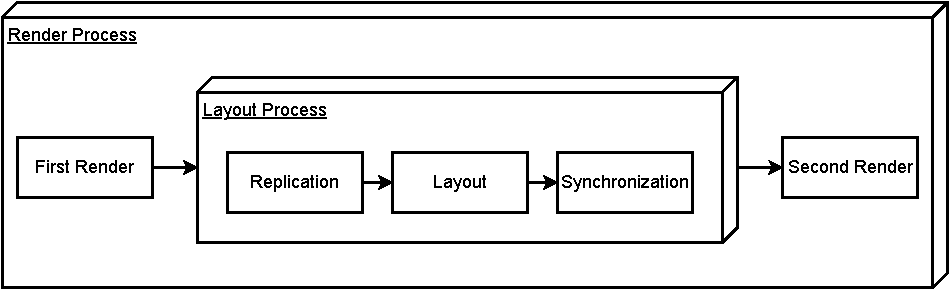
\includegraphics[keepaspectratio,width=\linewidth,height=\fullh]
{diagrams/respvis-render-process.pdf}
\caption[Render Process When Using the Layouter]{%
The three phases of the render process when using
the RespVis Layouter. During the first render phase, every element
that affects the layout needs to be rendered.  The layout phase of the
render process is equivalent to the layout process described in
Figure~\ref{fig:LayoutProcess}. In this phase, the Layouter
calculates the final positions and sizes of laid-out elements and
stores them in attributes on these elements.  During the second render
phase, the boundary informations calculated in the previous phase is
utilized to rerender all elements of the visualization at their final
positions with their final dimensions.  \imgcredit{Image created by
the author of this thesis using \href{https://diagrams.net/}{diagrams.net}.}
}
\label{fig:RenderProcess}
\end{figure}







\subsection{Axes}

Axes are implemented in the \code{axis.ts} file in the Core Module and
are used to visualize scales that map abstract values to spatial
dimensions. Currently, only Cartesian Axes, distinguished by their
position relative to a visualization's draw area, are provided by
RespVis, since only Cartesian Charts have been implemented so far.
The implementation has so far been focused on Left and Bottom Axes,
because they are the most commonly encountered types of Cartesian Axes
and cover most use cases. An Axis consists of ticks, an optional
title, and an optional subtitle, where the ticks of an Axis are the
actual visualization of the Axis' scale, and the title and subtitle
can be specified for additional description. An example of what a
rendered Left and Bottom Axis might look like can be seen in
Figure~\ref{fig:Axes}.

\begin{figure}[tp]
\centering
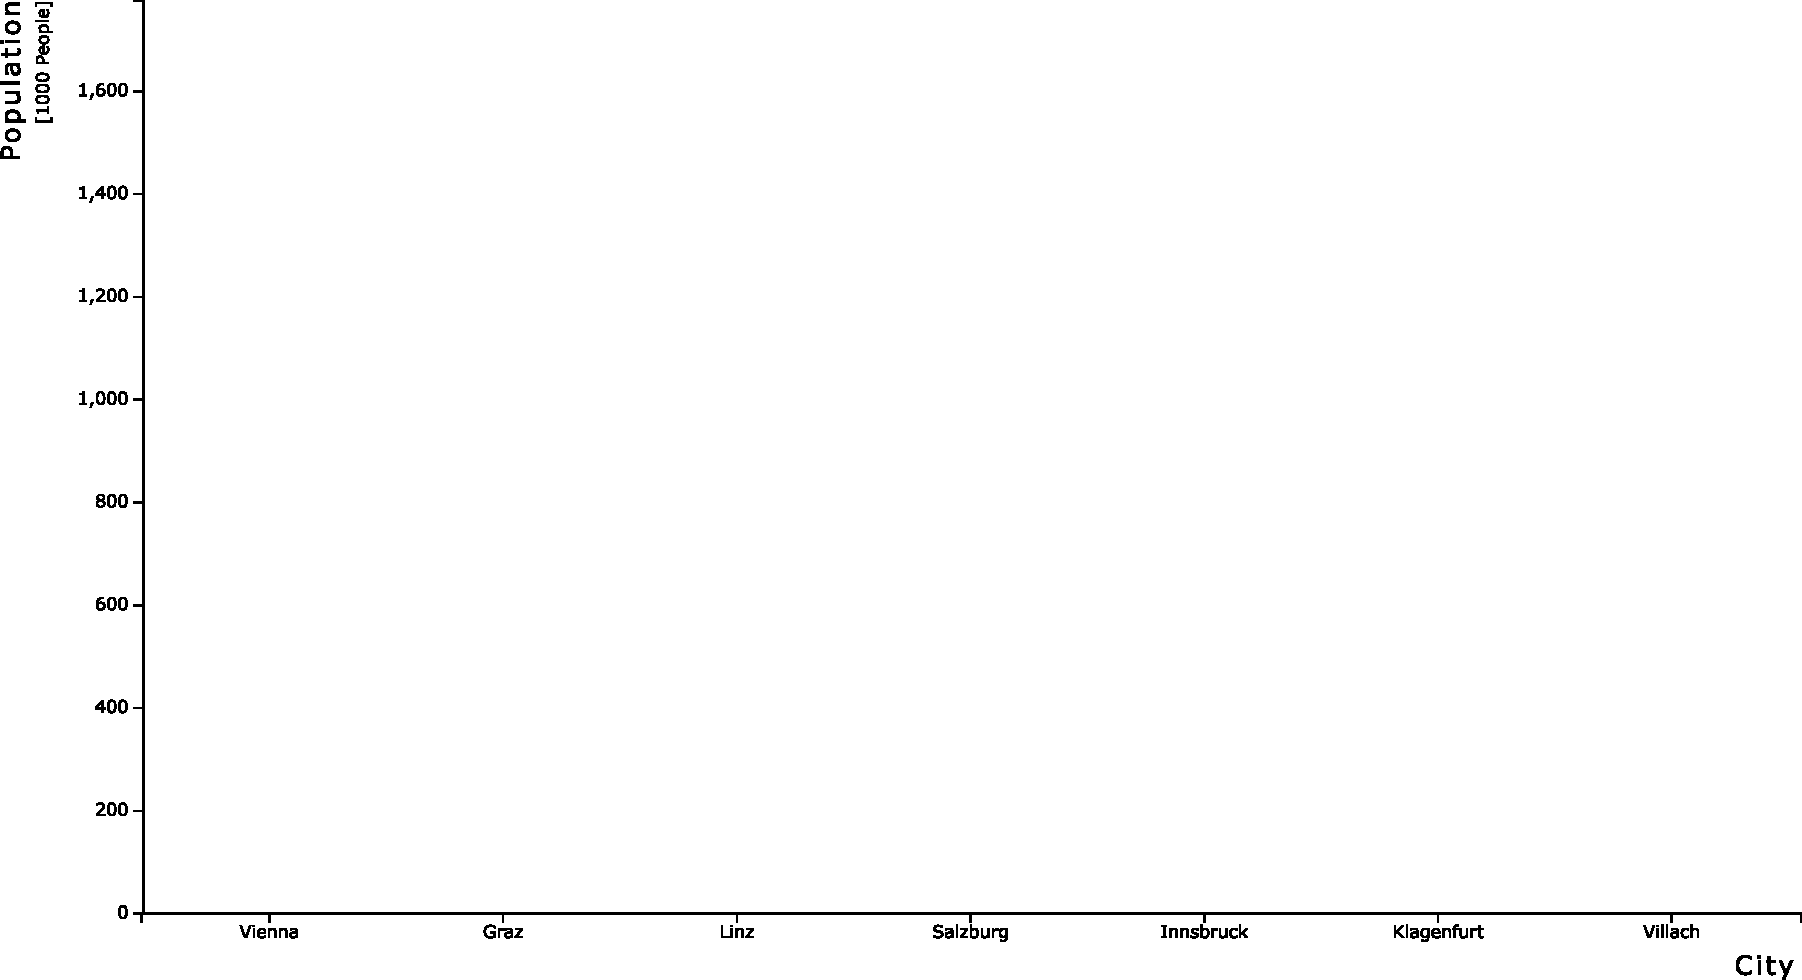
\includegraphics[keepaspectratio,width=\linewidth,height=\fullh]
{diagrams/axes.pdf}
\caption[RespVis Axis Components]{%
A rendered Left Axis with ticks, a title, and a subtitle, and a
Bottom Axis  with ticks and a title.
\imgcredit{Image created by the author of this thesis using RespVis
  and \href{https://inkscape.org/}{Inkscape}.}
}
\label{fig:Axes}
\end{figure}


The \code{Axis} interface describes the shape of a data object with
which an Axis can be configured.  It includes a \code{scale} property,
representing the scale to be visualized, the \code{title} and
\code{subtitle} string properties, and the \code{configureAxis}
function property, which can be used to configure the underlying D3
axis before rendering it. Like most other components, axis components
consist of two main functions: a data creation function and a render
function. The \code{axisData} function is used to create an
\code{Axis} data object from a \code{Partial<Axis>} object parameter,
where all non-set but required properties are filled with default
values. The \code{axisBottomRender} and \code{axisLeftRender}
functions are used to render a Left and Bottom Axis in a composite
element on which an \code{Axis} data object has been bound.  An Axis'
root element is a CSS Grid container and defines the layout of the
title, subtitle, and ticks elements.  The default configuration of a
Left Axis positions these elements in a three-column layout in which
the title, subtitle, and ticks elements are placed in this order from
left to right. For a Bottom Axis, the default configuration positions
the same elements in a three-row layout, in which the ticks, title,
and subtitle elements are placed in this order from top to bottom.
Furthermore, the title and subtitle elements of a Left Axis are
oriented vertically to save horizontal space using the
\code{textOrientation} utility function. Internally, the RespVis Axis
Components use the \code{axisBottom} and \code{axisLeft} functions
from the D3 Axis Module \parencite{D3Axis} to render the ticks of an
Axis. Since these D3 functions use attributes to position and style
elements, as many of these attributes as possible must be removed
directly after the ticks have been rendered to enable their
configuration via CSS.






\subsection{Chart}
\label{sec:Chart}

Charts are high-level components which represent a complete
visualization with Axes, Legends, and Series. An example of a rendered
RespVis Chart containing a Left Axis, a Bottom Axis, a Grouped Bar
Series, a Label Series, and a Legend can be seen in
Figure~\ref{fig:Chart}. A Chart is typically rendered in the root
\elname{<svg>} element of an SVG document that has at least the
\code{chart} class set in its \code{class} attribute and the
appropriate SVG namespace set in its \code{xmlns} attribute. These
attributes can be set in more specific Chart Components either
manually or via the \code{chartRender} function from the
\code{chart.ts} file in the Core Module, which only sets these
attributes.


\begin{figure}[tp]
\centering
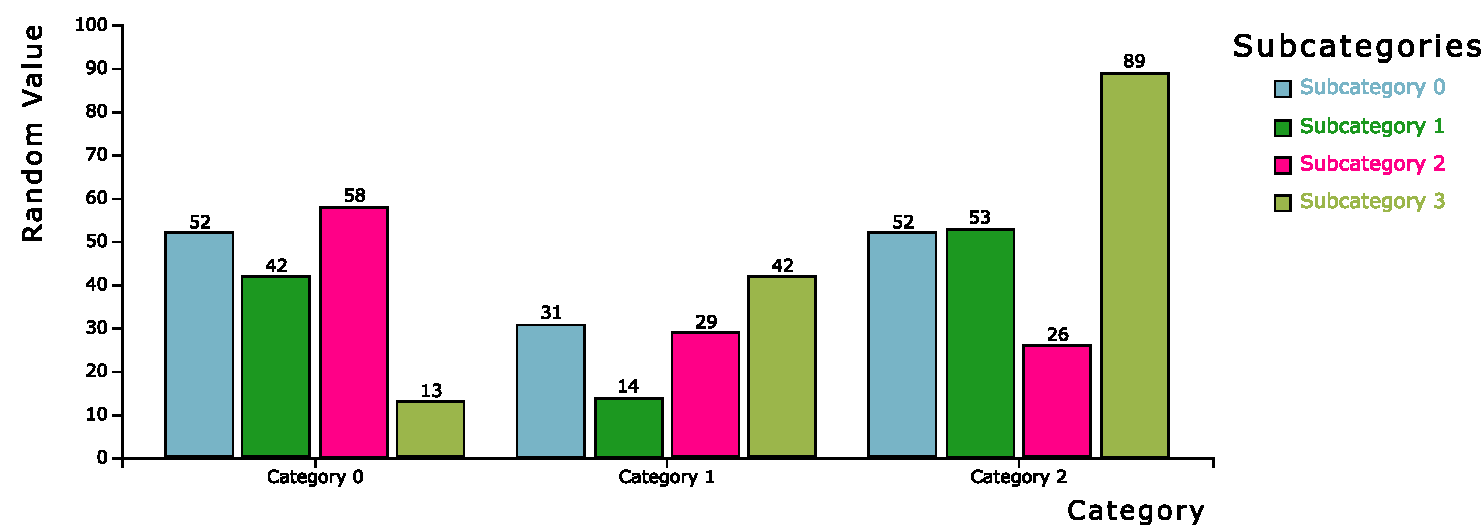
\includegraphics[keepaspectratio,width=\linewidth,height=\fullh]
{diagrams/chart.pdf}
\caption[Chart Example]{%
An example of a Chart containing a Left Axis, a Bottom Axis,
a Grouped Bar Series, a Label Series, and a Legend.
\imgcredit{Image created by the author of this thesis.}
}
\label{fig:Chart}
\end{figure}
% KA maybe need to annotate this figure to show the 5 components?


As mentioned previously, RespVis currently only supports Cartesian
Charts, which visualize data in a Cartesian coordinate system. The
implementation of the base functionality of  Cartesian Charts is
located in the \code{chart-cartesian.ts} file in the Core Module. The
\code{ChartCartesian} interface describes a data object for the
configuration of Cartesian Charts via the \code{xAxis} and
\code{yAxis} \code{Axis} properties which describe the X and Y Axes of
the Chart respectively. Transposing Axes is a useful pattern to
improve the responsiveness of visualizations and can be configured
using the \code{flipped} boolean property of \code{ChartCartesian}
data objects. If the \code{flipped} property is set to \code{false},
the \code{xAxis} object is used to configure the Bottom Axis and the
\code{yAxis} object is used to configure the Left Axis. If it is set
to \code{true}, it is the other way around.

The \code{chartCartesianData} function is used to create a
\code{ChartCartesian} data object. This function gets a partial data
object with only those properties set which are of interest to the
calling code, and all non-set properties are filled with default
values. The default values of the \code{xAxis} and \code{yAxis}
properties are set by the \code{axisData} function from the Axis
Module. The \code{flipped} property is initialized to \code{false}.

The rendering of Cartesian Charts is split into two functions which
have to be called separately, because not all parts of a Cartesian
Chart can be rendered simultaneously. The general structure of a Chart
must be rendered before anything else can be rendered, since this
includes the draw area container element into which individual Series
Components are rendered. A Chart's Axes need fully initialized scales
to be rendered correctly. However, the range of a scale, i.e. the
range of values into which abstract values are mapped, depends on the
size of the draw area and is only set during the render function of
the individual Series Components. Therefore, the Axes of a Cartesian
Chart must be rendered after Series Components in order to ensure
fully initialized scales.

The structure of a Cartesian Chart is rendered with the
\code{chartCartesianRender} function, which sets the necessary
attributes and classes on the root element and attaches the draw area
\elname{<svg>} element to it. The draw area is the container element
into which the Series Components of a Chart are rendered. An
\elname{<svg>} element without actual content is not able to receive
input events, which means that it would, for example, not be possible
to capture scroll events to control a zoom interaction when the cursor
is over the empty area of the draw area. To counter this, a
transparent \elname{<rect>} background element filling the whole draw
area is added, allows input events to be received even in empty areas.

The \code{chartCartesianAxesRender} function is used to render the
Axes of a Cartesian Chart. This function must only be called on
elements with a bound \code{ChartCartesian} data object and only after
the scales that are to be visualized by the Axes have been fully
initialized. Charts must first render the Chart's structure using the
\code{chartCartesianRender} function, followed by the desired Series
Components, and only then can the Chart's Axes be rendered using the
\code{chartCartesianAxesRender} function. The
\code{chartCartesianAxesRender} function creates two \elname{<g>}
elements and renders a Left Axis and a Bottom Axes in them. Depending
on whether the \code{flipped} property in the bound data object is set
to \code{true} or \code{false}, the \code{xAxis} data object is used
to configure the Bottom Axis or Left Axis and the \code{yAxis} data
object is used to configure the other. After the Axes are rendered,
the \code{x-axis} class is set on the one the \code{x-axis} data
object is bound to, and the \code{y-axis} class is set on the other
one.

The elements of a Cartesian Chart are positioned using a CSS Grid
layout. By default, a grid is created which defines the
\code{axis-left}, \code{axis-bottom}, \code{draw-area}, and
\code{legend} areas. Most rows and columns of this grid are sized to
fit their content, with the only exception being the row and column
containing the draw area, which is set to fill the remaining space not
occupied by the other rows and columns. The default CSS configuration
of a Cartesian Chart positions any legend to the right of the draw
area, but this can be changed by either adjusting the grid directly
via CSS or activating one of the preconfigured positions via the
\code{data-legend-position} attribute. To simplify setting the
\code{data-legend-position} attribute, the \code{chartLegendPosition}
function can be used, which sets this attribute to the value of the
passed \code{LegendPosition} enum parameter.






\subsection{Chart Window}

Chart Windows are implemented in the \code{chart-window.ts} file in
the Core Module and are wrapper components around Charts that render a
Chart inside a Layouter and decorate it with a Toolbar. These
components represent an even higher-level layer of abstraction than
Charts and are used to manage their rendering process and
configuration. In most other visualization libraries, Charts are
provided as the highest level of components that can be configured,
which typically means that additional HTML elements for the runtime
configuration of Charts have to be created and managed by the
embedding web page itself.  Chart Windows are rendered with the
\code{chartWindowRender} function on HTML \elname{<div>} elements
containing a Chart's SVG document.  Their structure consists of a
\elname{<div>} element in which the Toolbar is rendered, and of another
\elname{<div>} element on which a Layouter is initialized and which
holds the wrapped Chart's SVG document. An example of a Chart Window
with an expanded Tool Menu containing two Nominal Filtering Tools and
an SVG Download Tool can be seen in Figure~\ref{fig:ChartWindow}.


\begin{figure}[tp]
\centering
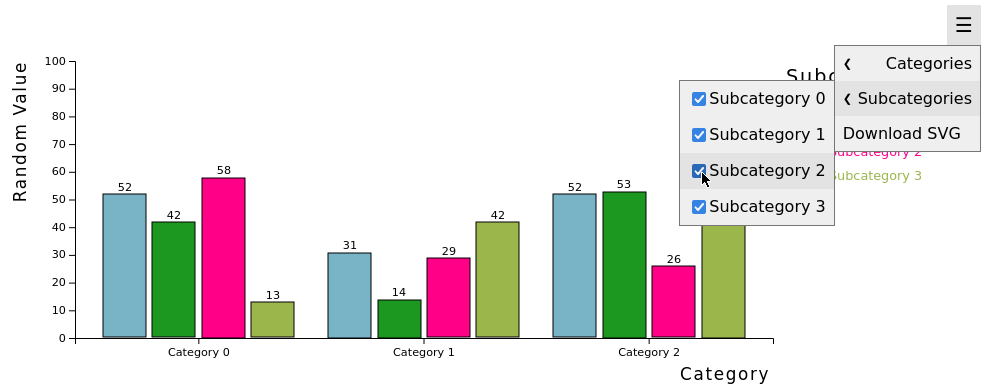
\includegraphics[keepaspectratio,width=\linewidth,height=\fullh]
{images/chart-window.png}
\caption[Chart Window Example]{%
An example of a Chart wrapped in a Chart Window. The Tool
Menu has been expanded by hovering over it, and the menu entries of
two Nominal Filtering Tools and the SVG Download Tool can be seen
inside. \imgcredit{Image created by the author of this thesis.}
}
\label{fig:ChartWindow}
\end{figure}


Currently, the Toolbar only contains the Tool Menu, a dropdown menu
into which individual tools are added as menu items or as submenus.
Dropdown menus are created with the \code{menuDropdownRender} function
and consist of a title and a container for menu items. The current
dropdown menu implementation uses no JavaScript and simply shows menu
items via CSS when there is a hover interaction. The Tool Menu is
created with the \code{menuToolsRender} function, which internally
uses the \code{menuDropdownRender} function to initialize it as a
dropdown menu.

The Core Module provides various tools which can be added to the Tool
Menu of Chart Windows. One of these tools is the Nominal Filtering
Tool located in the \code{tools/tool-filter-nominal.ts} file of the
Core Module. This tool is used to filter a nominal (or categorical)
data dimension of a visualized dataset via a dropdown menu that
includes a Checkbox Series. Nominal data, in contrast to ordinal or
quantitative data, consists only of labels that do not have a
quantitative value assigned to them and therefore have no inherent
ordering. The data object for the configuration of a Nominal Filter
Tool is described by the \code{ToolFilterNominal} interface, which
contains properties to specify the title of the dropdown menu, the
individual options to be filtered, and the keys of these options. The
\code{toolFilterNominalData} function is used to create a data object
of type \code{ToolFilterNominal} from a partial input object where
undefined properties are being filled with default values. Nominal
Filtering Tools can then be rendered on elements with bound
\code{ToolFilterNominal} data objects using the
\code{toolFilterNominalRender} function, which internally uses the
\code{menuDropdownRender} function to initialize a dropdown menu into
which the checkboxes representing the individual options of the filter
are rendered as menu items.

Checkbox Series are implemented in the \code{series-checkbox.ts} file
in the Core Module and render a series of checkboxes consisting of
checkbox \elname{<input>} elements with associated \elname{<label>}
elements. They are configured using data objects in the form of the
\code{SeriesCheckbox} interface, which contains properties to
determine the type of checkbox container elements and the labels of
checkboxes. A data object of this type can be created with the
\code{seriesCheckboxData} function, which creates a complete object
from a partial one. Checkbox Series are rendered using the
\code{seriesCheckboxRender} function, which generates individual
checkboxes using a data join requiring an array of \code{Checkbox}
data objects so that a single data object can be bound to each
checkbox. Individual \code{Checkbox} data objects contain all the data
needed to render a single checkbox and are created by transforming the
\code{SeriesCheckbox} data objects bound on the Series' root element.
Single checkboxes consist of a container element, an \elname{<input>}
checkbox element, and a \elname{<label>} element. In order to
semantically assign the \elname{<label>} elements to their
\elname{<input>} elements, the \code{for} attributes on \elname{<label>}
elements must be set to the ids of their corresponding \elname{<input>}
elements. This requires assigning unique ids to \elname{<input>}
elements, which are generated via the \code{uuid} function and set as
\code{id} attributes on the \elname{<input>} elements and as \code{for}
attributes on \elname{<label>} elements when the checkbox is first
created. The \code{uuid} function is an alias for the \code{v4}
function from the \code{uuid} npm package \parencite{UUIDPackage} and
is used to generate UUIDs (Universally Unique IDentifiers)
\parencite{UUIDRFC} of the fourth version, which are very likely to be
unique and therefore can be safely used as values for \code{id}
attributes.

The SVG Download Tool is implemented in the
\code{tools/tool-download-svg.ts} file of the Core Module and is
included by default in every Chart Window. SVG documents embedded in
HTML documents cannot be downloaded by web consumers as easily as
raster images, which can simply be downloaded with native browser
tools. Instead, SVG documents must be encoded in \code{Blob} objects
and then set as as object URLs in the \code{href} attributes of
\elname{<a>} elements. However, since the presentation of RespVis
visualizations is mainly configured using CSS, the active CSS
properties must first be converted to attributes before the SVG
document can be downloaded. For this, a clone of the whole SVG
document is made to set attributes on the cloned elements without
affecting the rendered visualization. After the document has been
cloned, attributes reflecting the active CSS configuration of the
original elements are set on cloned elements. The active CSS
configuration of the original elements is calculated using the
\code{elementComputedStyleWithoutDefaults} utility function, which
yields a list of CSS properties and their values, only containing
properties that are not set to defaults. After setting all the
necessary attributes on cloned elements, the string representation of
the cloned document is calculated using the \code{Element.innerHTML}
property and encoded in a \code{Blob} object with the content type
\code{image/svg+xml}. At present, the string representation of the SVG
document is not processed further or prettily formatted, which results
in a rather difficult-to-read file and which will be improved in
future work. The \code{Blob} object containing the SVG document is
further transformed into an object URL via the
\code{URL.createObjectURL} method and set in the \code{href} attribute
of a newly created \elname{<a>} element. This newly created
\elname{<a>} element is then briefly attached to the \elname{<body>}
element of the active HTML document and clicked using the
\code{Element.click} method, which initiates the download of the final
prepared SVG document. Download SVG Tools can be rendered as menu
items in a Chart Window's Tool Menu with the
\code{toolDownloadSVGRender} function, which initializes them and
triggers the download of the SVG document embedded in the Chart Window
when a visualization consumer clicks on the menu item.





\section{Legend Module}

The Legend Module in the \code{src/lib/legend/} directory currently
comprises a sigle file \code{legend.ts}, containing the implementation
of the Legend Component. Legends are used to visualize scales whose
abstract values are not mapped to spatial dimensions in a coordinate
system, but to other visual properties such as colors, shapes, or
sizes. The Legend implemented in this module illustrates such scales
by creating labeled, configurable symbols for every mapping and,
therefore, this component is best suited for the visualization of
discrete value mappings. Continuous data dimensions can still be
visualized with this component, but they must be approximated by
dividing the continuous domain of values into equal discrete steps.
An example demonstrating the use of the Legend Module can be found in
the \code{legend.html} file in the \code{src/examples/} folder. An
excerpt from this example can be seen in Listing~\ref{list:Legend},
with its rendering shown in Figure~\ref{fig:Legend}.

\begin{samepage}
\lstinputlisting[%
  float=tp,
  aboveskip=\floatsep,
  belowskip=\floatsep,
  xleftmargin=0cm,              % no extra margins for floats
  xrightmargin=0cm,             % no extra margins for floats
  %
  basicstyle=\footnotesize\ttfamily,
  frame=shadowbox,
  numbers=left,
  label=list:Legend,
  caption={[Source Code of Legend Example]%
The source code of the example implemented in the \code{legend.html}
file in the \code{src/examples/} directory. When executed, this code
results in the three Legends shown in Figure~\ref{fig:Legend}.
Non-essential parts of the source code have been removed to focus on
Legend-related configurations. The horizontal Legend is configured
with the same data object as the rectangle symbol Legend, but the
items of the horizontal Legend are laid out horizontally via the
\code{flex-direction: row} CSS property.
},
]{listings/legend.html}
\end{samepage}



\begin{figure}[tp]
\centering
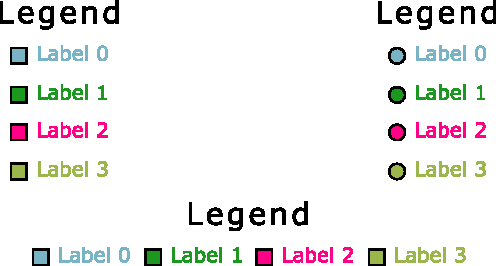
\includegraphics[keepaspectratio,width=\linewidth / 2,height=\fullh]
{diagrams/legend.pdf}
\caption[Legend Example]{%
The three Legends resulting from the source code in
Listing~\ref{list:Legend}. The first Legend has been configured to have
rectangles as symbols, the second to have circles as
symbols, and the third with rectangle symbols horizontally laid out.
\imgcredit{Image created by the author of this thesis.}
}
\label{fig:Legend}
\end{figure}



A data object for the configuration of a Legend is defined by the
\code{Legend} interface, which contains properties to describe the
title, labels, and symbols of a Legend. Symbols are configured via
functions which take the boundaries calculated by the Layouter into
account to set the \code{d} attributes of \elname{<path>} elements.
Legend symbols are rendered as \elname{<path>} elements because these
enable the rendering of arbitrary symbols that can be changed
dynamically, whereas the usage of \elname{<rect>} or \elname{<circle>}
elements would be much more restrictive. A disadvantage of using
\elname{<path>} elements is that, since they require manual
configuration of exact shapes via path definition strings, their usage
is more tedious than the usage of more restricted SVG elements, and
they require slightly more annotation effort when it comes to
accessibility. Colors of individual items in a Legend are indirectly
configured via \code{data-style} attributes on items whose values are
specified in the \code{Legend} data objects. Some style classes, such
as the \code{categorical-x} classes for categorical styling, are
already provided by RespVis and handled in the library's distributable
CSS file. Furthermore, custom style classes can easily be added by
simply handling them in custom CSS rules. \code{Legend} data objects
can be created with the \code{legendData} function, which receives a
partial input object in which the properties which are not of interest
to the calling code are not required to be set and are populated with
default values.

A Legend is rendered into elements which have a \code{Legend} data
object bound on them using the \code{legendRender} function. This
function sets the \code{legend} class on the root element, attaches a
\elname{<text>} element with which the title of the Legend is shown, and
attaches a \elname{<g>} element into which the individual items of the
Legend are rendered via a data join. To perform the data join with
which the items of the Legend are created, one \code{LegendItem} data
object per item to be rendered is needed to describe individual legend
items, and these are generated via transformation of the bound
\code{Legend} data object. Via a data join with these data objects,
one \elname{<g>} element with the \code{legend-item} class is created
for every legend item, to which a \elname{<path>} element for the symbol
and a \elname{<text>} element for the associated label are attached.
The operations performed during this data join can be directly
modified via the custom \code{enter}, \code{update}, and \code{exit}
events, which are dispatched on the root element of the Legend and
which respectively contain the data join's enter, update, or exit
selection in a property of the event object. Also, the
\code{legendRender} function sets the \code{data-style} and
\code{data-key} attributes on the legend item elements to values
configured on the bound \code{Legend} data object.






\section{Tooltip Module}
\label{sec:TooltipModule}

Tooltips display additional contextual information which is too
expansive to be shown all the time. The more information a
visualization shows simultaneously, the more cognitive effort is
required to interpret it. Detailed information which may be valuable
but is not absolutely necessary for understanding a visualization's
core message is only shown via a Tooltip when a visualization consumer
interacts with an element in whose context this information stands.
Since Tooltips are only shown explicitly after consumer interaction, they
may overlap and cover other elements of a Chart which would otherwise
be too important to hide. An example of a Bar Chart in which
additional information is displayed via a Tooltip can be seen in
Figure~\ref{fig:Tooltip}.


\begin{figure}[tp]
\centering
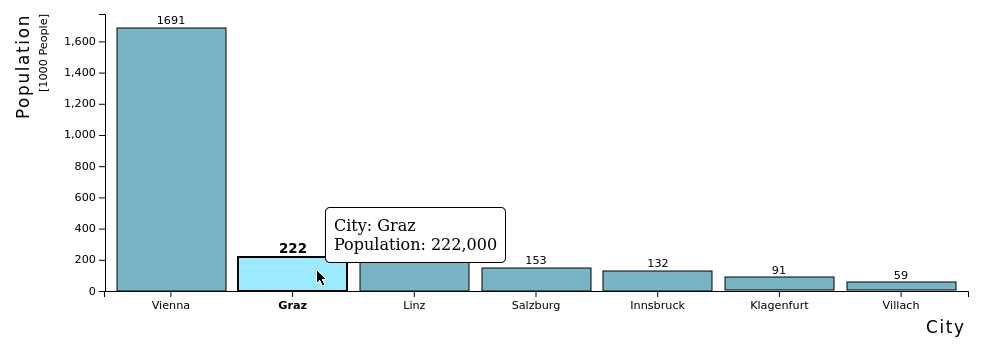
\includegraphics[keepaspectratio,width=\linewidth,height=\fullh]
{images/tooltip.png}
\caption[Tooltip Example]{%
A Bar Chart with an active Tooltip displaying
additional information from the data record associated with an
individual bar. Since a Tooltip is only visible during
interaction with a particular element, it may sometimes overlap
and cover other important parts of a Chart.
\imgcredit{Image created by the author of this thesis.}
}
\label{fig:Tooltip}
\end{figure}


The Tooltip Module is located in the \code{src/lib/tooltip/} directory
of the RespVis library and contains the implementation of Tooltips and
utility functions to simplify the configuration of Tooltips on Series
Components. Tooltips are merely HTML \elname{<div>} elements with the
\code{tooltip} class, which are styled via CSS and which can be
initialized with the \code{tooltip} function. Their visibility,
position, and content is controlled via the \code{tooltipShow},
\code{tooltipHide}, \code{tooltipPosition}, and \code{tooltipContent}
functions in the \code{tooltip.ts} file of the Tooltip Module. Since
RespVis supports multiple simultaneous Tooltips, all of these
functions have to be passed the Tooltip element they should affect.
Alternatively, passing a \code{null} value operates on the default
Tooltip. Tooltips are shown and hidden via the \code{tooltipShow} and
\code{tooltipHide} functions, which respectively add or remove the
\code{show} class to the classes of the Tooltip element. The actual
showing and hiding is done in CSS by setting the \code{opacity}
property of the element depending on whether or not the \code{show}
class is set. Positions of Tooltips are configured via the
\code{tooltipPosition} function.  This function calculates positions
through an anchor position in viewport coordinates and a directional
offset from that anchor.  Specifying the anchor position is necessary,
but the directional offset can be omitted to have a sensible one
chosen by the \code{tooltipPosition} function, so that the Tooltip is
always placed inside the visible area of the browser. The actual
positioning is again done in CSS by setting a combination of the
\code{left}, \code{right}, \code{bottom}, and \code{top} properties
depending on the offset direction of the Tooltip. A Tooltip's content
can be set with the \code{tooltipContent} function, which sets the
Tooltip's inner HTML to the HTML string passed to the function.

Apart from Tooltips, the Tooltip Module also contains utility
functions to simplify the setup and handling of Tooltips on
different Series Components such as Bar or Point Series. Interfaces
describing the data objects of Series Components can inherit from the
\code{SeriesConfigTooltips} interface to add additional properties for
the configuration of Tooltips to these data objects. Among these
properties is a property to enable the Tooltips of the Series and
properties to specify the contents and positions of individual
Tooltips based on their associated context-element and the current
cursor position. In addition to the \code{SeriesConfigTooltips}
interface, the \code{seriesConfigTooltipsHandleEvents} function is
provided to automatically set \code{mouseover}, \code{mousemove}, and
\code{mouseout} event listeners on Series to automatically update the
visibility, content, and position of Tooltips based on the
\code{SeriesConfigTooltips} properties stored in the Series' data
object. The usage of these utilities is optional, and Series
Components are free to provide their own properties for the
configuration of Tooltips and their handling. However, for
consistency reasons, the way of configuring Tooltips should not differ
too much between different types of Series Components, and therefore
it is recommended to use the utilities provided here unless there is a
good reason not to.





\section{Bar Module}

A bar chart is used to compare the values of a quantitative variable
(values) uniquely associated with the distinct values of a qualitative
variable (categories), using labelled rectangles whose lengths are
proportional to the values. Examples of datasets suitable for plotting
with a bar chart would be countries with their populations, people
with their ages, and web browsers with their market shares. Bar charts
have been in use for many centuries, with one of the earliest
documented occurrences being \textcite{CommercialAndPoliticalAtlas},
and are among the most frequently encountered types of visualizations
in the modern web.

The bars of a bar chart can be either horizontally or vertically
oriented. In horizontal bar charts, sometimes also called row charts,
categories are spread in equal intervals across the y-axis to define
the positions and heights of bars, and the associated values of
categories are mapped on the x-axis to determine their widths.
Conversely, in vertical bar charts, sometimes also called column
charts, categories are spread in equal intervals across the x-axis to
determine the positions and widths of bars, and the values of
categories are mapped on the y-axis to determine their heights.
Horizontal bar charts are better suited for display in narrow contexts
than vertical bar charts, because category labels can be positioned
more easily without having to rotate them and because these charts can
be vertically extended by having visualization consumers scroll
vertically, which is strongly preferable to scrolling horizontally.


The Bar Module is located in the \code{src/lib/bars/} directory of the
RespVis library and contains components to create Single-Series,
Grouped Multi-Series, and Stacked Multi-Series Bar Charts that can be
used in different situations. For every type of Bar Chart, the Bar
Module provides a respective Series Component to render only the
actual bars, a Chart Component to render a full Chart including bars,
axes, and possible legends, and a Chart Window Component to render a
full Chart embedded into a Layouter with additional tools provided via
a Toolbar. Higher-level components are more convenient to use, but
they also impose more assumptions, and therefore restrictions, on
lower-level components contained within them. The implementations of
the different types of Bar Charts and when to best use which type is
described in the following sections.





\subsection{Single-Series Bars}

Single-series bar charts are what most people think of when thinking
of bar charts. They consist of only a single series of bars and can
therefore only visualize differences between categories associated
with a single quantitative value at a time. The categories of a
single-series bar chart are mapped to spatial dimensions via a band
scale which partitions available space into equal intervals (bands)
with configurable padding between them. Thus, the width of bars is
calculated via the total number of categories, the range they are
spread on, and the padding between them. The mapping of quantitative
values to spatial dimensions in a single-series bar chart is performed
using a continuous scale which maps quantitative values stored in a
dataset into a range of values between two extremes via a continuous
interpolation function. In most cases, linear interpolation via a
linear scale is used to map quantitative values, but visualization
authors can choose other forms of interpolation, such as logarithmic
interpolation via a logarithmic scale.

In RespVis, the Bar Series module renders collections of \elname{<rect>}
elements representing the bars in a Bar Chart's draw area, and they
are the lowest-level components required for rendering Bar
Charts. Their implementation is located in the \code{series-bar.ts}
file of the Bar Module and contains the \code{SeriesBar} interface
describing data objects to configure Bar Series, the
\code{seriesBarData} function to create these data objects from
partial data objects, and the \code{seriesBarRender} function to
render Bar Series. The \code{SeriesBar} interface inherits Tooltip
configuration properties from the \code{SeriesConfigTooltips}
interface described in Section~\ref{sec:TooltipModule} and adds
additional properties to configure the used categories and values, the
scales to map them to spatial dimensions, whether or not bars should
be oriented vertically or horizontally, and properties to configure
their colors and keys.  After the desired \code{SeriesBar} data
objects have been created and bound to \elname{<svg>} or \elname{<g>}
elements, the \code{seriesBarRender} function can be used to render
Bar Series on these elements. During rendering, the bound
\code{SeriesBar} data object is transformed into an array of
\code{Bar} data objects, and a data join with these data objects is
performed to render the individual bars. The output range of the
scales used to map categories and values to spatial dimensions is set
to the dimensions of the Bar Series element's bounding box that has
been previously calculated and stored in the \code{bounds} attribute
by the Layouter.  With these scales, the dimensions of bars are
calculated, and enter, update, and exit transitions are utilized to
interpolate them towards these new dimensions, so that changes in
visualization are easier to track, which leads to an improved
experience for visualization consumers. As with all other Series, the
\code{enter}, \code{update}, and \code{exit} events containing the
respective data join selections are dispatched on the Series' root
element and allow the injection of custom behavior into the different
phases of the Series' data join.

Bar Charts are Cartesian Charts, as discussed in
Section~\ref{sec:Chart}, which display a Bar Series with optional
labels in their draw area and render the scales used to map categories
and values to spatial dimensions as Axes. Their implementation can be
found in the \code{chart-bar.ts} file of the Bar Module, which
contains the \code{ChartBar} interface to describe data objects used
for the configuration of Bar Charts, the \code{chartBarData} function
to create a fully initialized \code{ChartBar} data object from a
partial input object, and the \code{chartBarRender} function to render
Bar Charts as \elname{<svg>} or \elname{<g>} elements to which
\code{ChartBar} data objects have been bound. The \code{ChartBar}
interface inherits all properties of the \code{ChartCartesian} and
\code{SeriesBar} interfaces and adds additional properties for the
configuration of bar labels. It is not necessary to manually specify
all the offered properties of this interface because the
\code{chartBarData} function initializes all of them with sensible
defaults derived from the properties callers are interested in and
which have been specified in the partial data object passed to this
function. The \code{chartBarRender} function simply initializes a
Cartesian Chart and renders a Bar Series whose configuration is
derived from the \code{ChartBar} data object bound to the Chart's
element and an optional series of labels to annotate the bars of the
Bar Series into the Cartesian Chart's draw area. Furthermore, the
scales used for rendering the Bar Series are visualized as Left and
Bottom Axes of the Cartesian Chart, and a \code{mouseover} event
listener to highlight bars and their corresponding ticks on the
category axis is attached to bars.

Bar Chart Windows are high-level components which wrap a Bar Chart
into a Layouter so its elements can be laid out with CSS. They also
add a Toolbar containing tools to filter a Bar Chart's categories and
download an SVG version of the current chart. Their implementation can
be found in the \code{chart-window-bar.ts} file of the Bar Module,
which contains the \code{ChartWindowBar} interface to describe data
objects for the configuration of Bar Chart Windows, the
\code{chartWindowBarData} function to create a fully initialized
\code{ChartWindowBar} data object from a partial input object
containing only relevant properties, and the
\code{chartWindowBarRender} function to render a Bar Chart Window as a
\elname{<div>} element onto which a \code{ChartWindowBar} data object
has been bound. The \code{ChartWindowBar} interface inherits all
properties of the \code{ChartBar} interface to configure the wrapped
Bar Chart and adds additional properties needed for the filtering of
categories. Bar Chart Windows are rendered with the
\code{chartWindowBarRender} function, which renders a Toolbar
including a Nominal Filtering Tool for categories and an SVG Download
Tool, initializes the nested Bar Chart with the filtered values, and
renders it, according to the render process required by the Layouter
defined in Section~\ref{sec:Layouter}.


\begin{samepage}
\lstinputlisting[%
  float=tp,
  aboveskip=\floatsep,
  belowskip=\floatsep,
  xleftmargin=0cm,              % no extra margins for floats
  xrightmargin=0cm,             % no extra margins for floats
  %
  basicstyle=\footnotesize\ttfamily,
  frame=shadowbox,
  numbers=left,
  label=list:BarChartWindow,
  caption={[Bar Chart Window Example]%
The example source code to create the Bar Chart Window shown in
Figure~\ref{fig:BarChartWindow}. This Bar Chart Window is configured
with the bound data object initialized with the
\code{chartWindowBarData} function and rendered with the
\code{chartWindowBarRender} function. Since no special responsive
behavior is desired in this example, the default resize and category
filter behavior is attached to the Chart Window via the
\code{chartWindowBarAutoResize} and
\code{chartWindowBarAutoFilterCategories} functions.
},
]{listings/bar-chart-window.js}
\end{samepage}


By default, Bar Chart Windows are not automatically updated when the
viewport size changes or if their categories are filtered. Instead, a
custom \code{resize} event listener is attached to the Chart Window's
element, in which the Chart Window is responsively reconfigured
according to the changed viewport size and subsequently rerendered via
the \code{chartWindowBarRender} function. Furthermore, Bar Chart
Windows dispatch custom \code{categoryfilter} events containing the
currently active categories whenever categories are activated or
deactivated via the Nominal Filtering Tool. These events can be used
to responsively reconfigure Bar Chart Windows according to the
currently active categories by adding a custom \code{categoryfilter}
event listener which updates the configuration of the Bar Chart Window
accordingly and rerenders it. If no special configuration is required
when the viewport size or the category filtering changes, then the
\code{chartWindowBarAutoResize} and
\code{chartWindowBarAutoFilterCategories} functions can be used to
attach custom \code{resize} and \code{categoryfilter} event listeners
to implement the default behavior. A simple example of how a scalable
Bar Chart Window with filterable categories can be created is shown in
Listing~\ref{list:BarChartWindow} and the resulting visualization is
shown in Figure~\ref{fig:BarChartWindow}.



\begin{figure}[tp]
\centering
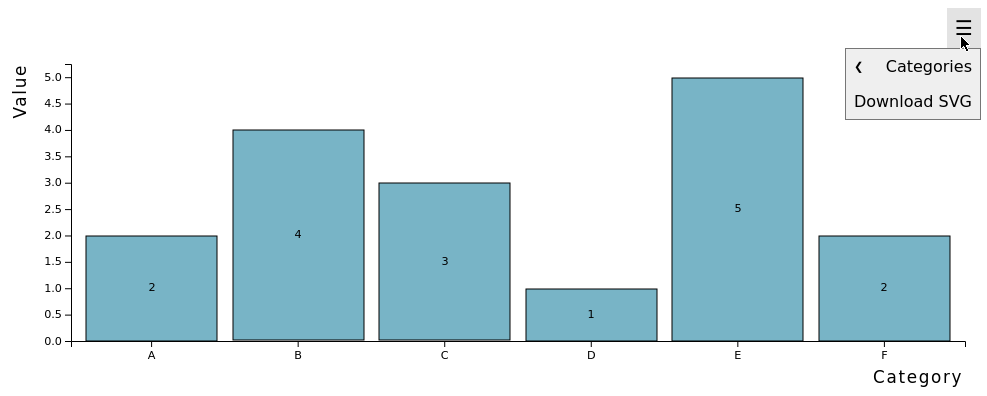
\includegraphics[keepaspectratio,width=\linewidth,height=\halfh]
{images/bar-chart-window.png}
\caption[Bar Chart Window Example]{%
The Bar Chart Window resulting from the example code in
Listing~\ref{list:BarChartWindow}.
\imgcredit{Image created by the author of this thesis using RespVis.}
}
\label{fig:BarChartWindow}
\end{figure}






\subsection{Grouped Bars}

Grouped bar charts, sometimes also called clustered or multi-series
bar charts, consist of multiple series of bars and are used to
visualize differences between categories where each category is
associated with a number of quantitative variables. Every category
must be associated with the same number of quantitative variables,
effectively splitting categories into subcategories, and all values
assigned to these subcategories must be comparable with one another,
meaning they must have the same units and scales. As with
single-series bar charts, categories in grouped bar charts are also
mapped to spatial dimensions using band scales, but here, two
different band scales have to be applied. The category band scale
divides the available space along either the x or y-axis into
equal intervals based on the number of categories, whereas the
subcategory band scale further divides these intervals into even
smaller intervals based on the number of subcategories. Quantitative
values are again mapped to spatial dimensions via a single continuous
scale which must be used for all of them.

In RespVis, the Bar Module provides the Grouped Bar Series, Grouped
Bar Chart, and Grouped Bar Chart Window Components, which are very
similar to their Single-Series Bar Chart counterparts, to render
grouped bar charts in different levels of hierarchy. Grouped Bar
Series are the lowest-level components of these and render a
collection of \elname{<rect>} elements meant for display in the draw
area of a Grouped Bar Chart. The difference between a Grouped Bar
Series and a Single-Series Bar Series is that this one offers
additional properties needed for the configuration of subcategories
and that other properties specified as one-dimensional arrays in
Single-Series Bar Series are here required to hold two-dimensional
arrays so that their values can be assigned to the two-dimensionally
grouped bars. All bars belonging to the same subcategory have the same
style to simplify their comparison across all categories. Grouped Bar
Charts are Cartesian Charts which contain a Grouped Bar Series with
optional labels in their draw area, Left and Bottom Axes that
visualize the scales used by this Grouped Bar Series, and a Legend
that describes the different subcategories. These Charts also attach
event listeners to various elements to highlight bars, labels, ticks
on the category axis, and Legend items that semantically belong
together.

Grouped Bar Chart Windows are the highest-level components to render
visualizations based on Grouped Bars. They contain Grouped Bar Charts
wrapped inside Layouters and render them following the render process
defined in Section~\ref{sec:Layouter} to allow positioning of their
elements via CSS. Furthermore, they decorate their nested Charts with
Toolbars containing tools to download them as SVG documents and filter
their categories and subcategories. Every time a visualization
consumer interacts with these Nominal Filtering Tools to change the
configuration of displayed categories and subcategories, the
\code{categoryfilter} and \code{subcategoryfilter} events are
dispatched, containing the newly active categories and subcategories
respectively. Visualization authors can either implement special
resize and filter behavior by attaching custom listeners to these
events, or can activate the default behavior via the
\code{chartWindowBarGroupedAutoResize},
\code{chartWindowBarGroupedAutoFilterCategories}, and
\code{chartWindowBarGroupedAutoFilterSubcategories} functions. Example
code to create a scalable Grouped Bar Chart Window whose categories
and subcategories can be filtered via the Toolbar is shown in
Listing~\ref{list:GroupedBarChartWindow} and the resulting
visualization is shown in Figure~\ref{fig:GroupedBarChartWindow}.



\begin{samepage}
\lstinputlisting[%
  float=tp,
  aboveskip=\floatsep,
  belowskip=\floatsep,
  xleftmargin=0cm,              % no extra margins for floats
  xrightmargin=0cm,             % no extra margins for floats
  %
  basicstyle=\footnotesize\ttfamily,
  frame=shadowbox,
  numbers=left,
  label=list:GroupedBarChartWindow,
  caption={[Grouped Bar Chart Window Example]%
Example source code to create the Grouped Bar Chart Window shown in
Figure~\ref{fig:GroupedBarChartWindow}. The Grouped Bar Chart Window
is configured via a bound data object which is initialized with the
\code{chartWindowBarGroupedData} function and rendered with the
\code{chartWindowBarGroupedRender} function. Since no special
responsive behavior is desired in this example, the default resize,
category filter, and subcategory filter behavior is attached to the
Chart Window via the \code{chartWindowBarGroupedAutoResize},
\code{chartWindowBarGroupedAutoFilterCategories}, and
\code{chartWindowBarGroupedAutoFilterSubcategories} functions.
},
]{listings/grouped-bar-chart-window.js}
\end{samepage}


  
\begin{figure}[tp]
\centering
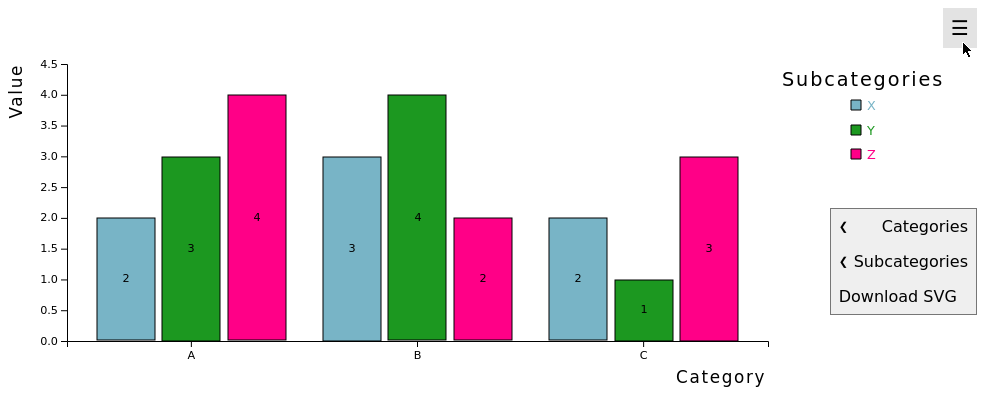
\includegraphics[keepaspectratio,width=\linewidth,height=\fullh]
{images/grouped-bar-chart-window.png}
\caption[Grouped Bar Chart Window Example]{%
The Grouped Bar Chart Window resulting from the example source code in
Listing~\ref{list:GroupedBarChartWindow}. The Tool Menu popup has
been manually displaced to not cover the legend.
\imgcredit{Image created by the author of this thesis using RespVis.}
}
\label{fig:GroupedBarChartWindow}
\end{figure}








\subsection{Stacked Bars}

Stacked bar charts are multi-series bar charts in which individual
series of bars are rendered as stacks rather than as clusters. Since
the bars of stacked bar charts do not share a common baseline, these
charts are not well-suited for comparing individual subcategories
across multiple categories but rather for approximating the
contributions of subcategories to the totals of their categories. A
bar's color is determined by its subcategory so that all bars that
have the same subcategory are colored equally. Percent stacked bar
charts are variants of stacked bar charts, in which the totals of all
categories are transformed to equal 100\% using the quantitative
values of subcategories as ratios of a whole. Due to this
transformation, all stacks of bars are of equal length, meaning the
information about their totals is lost, but the share subcategories
contribute to their categories is emphasized more strongly than in
ordinary stacked bar charts. Bar stacks are created by splitting the
category axis into equal intervals via a band scale into which bars
representing the different subcategories are stacked on top of one
another. The lengths of stacked bars are proportional to their
quantitative values and are calculated via a continuous scale which
maps these values into the range of the value axis.


The RespVis library provides a Series, a Chart, and a Chart Window
Component to render Stacked Bar Charts, all of which are highly
similar to their Grouped Bar counterparts. Bars in Stacked Bar Series
are grouped two-dimensionally (category/subcategory), and
configuration properties affecting individual bars are specified as
two-dimensional arrays. The main difference between Stacked Bar Series
and Grouped Bar Series lies in how the positions and extents of bars
are calculated. Stacked Bar Charts are, just like Grouped Bar Charts,
Cartesian Charts consisting of a Stacked Bar Series with optional
labels, two Axes, and a Legend. Furthermore, Stacked Bar Chart Windows
are also equivalent to Grouped Bar Chart Windows as they wrap a
Stacked Bar Chart into a Layouter, manage their render process, and
decorate it with a Toolbar containing two Nominal Filtering Tools to
filter categories and subcategories. Percent Stacked Bar Charts can be
rendered either by directly setting percentual values that lead to all
category totals summing up to 100\% or by enabling the
\code{valuesAsRatios} configuration property, which causes
quantitative values to be treated as ratios which are transformed to
percentual shares of their category totals during rendering.
Listing~\ref{list:StackedBarChartWindow} shows example RespVis
code to create a scalable Stacked Bar Chart Window whose categories
and subcategories can be filtered, the chart itself is shown in
Figure~\ref{fig:StackedBarChartWindow}.
 

\begin{samepage}
\lstinputlisting[%
  float=tp,
  aboveskip=\floatsep,
  belowskip=\floatsep,
  xleftmargin=0cm,              % no extra margins for floats
  xrightmargin=0cm,             % no extra margins for floats
  %
  basicstyle=\footnotesize\ttfamily,
  frame=shadowbox,
  numbers=left,
  label=list:StackedBarChartWindow,
  caption={[Stacked Bar Chart Window Example]%
Example source code to create the Stacked Bar Chart Window shown in
Figure~\ref{fig:StackedBarChartWindow1}. The Stacked Bar Chart Window
is configured with the bound data object initialized via the
\code{chartWindowBarStackedData} function and rendered with the
\code{chartWindowBarStackedRender} function. Since no special
responsive behavior is desired in this example, the default resize,
category filter, and subcategory filter behavior is attached to the
Chart Window via the \code{chartWindowBarStackedAutoResize},
\code{chartWindowBarStackedAutoFilterCategories}, and
\code{chartWindowBarStackedAutoFilterSubcategories} functions.
Setting the \code{valuesAsRatios} variable to \code{true}
would result in the Percent Stacked Bar Chart shown in
Figure~\ref{fig:StackedBarChartWindow2}.
},
]{listings/stacked-bar-chart-window.js}
\end{samepage}





\begin{figure}[tp]
\centering
\subfloat[Stacked Bar Chart]{%
\hspace{1cm}
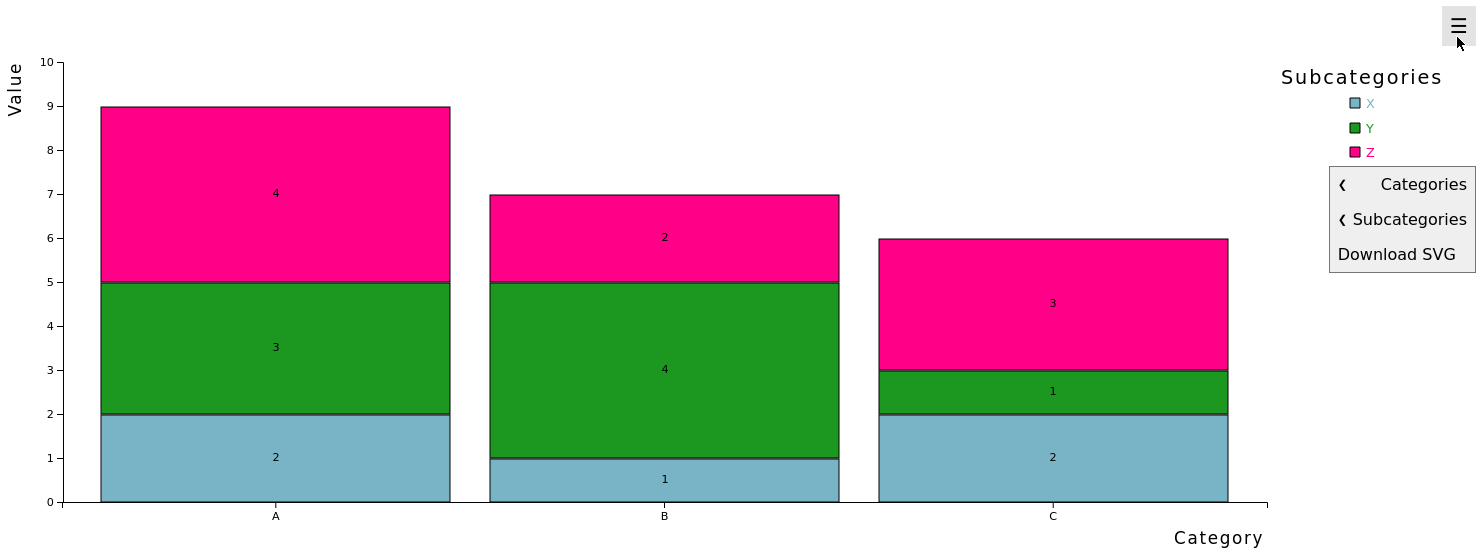
\includegraphics[keepaspectratio,width=\linewidth,height=\halfh]
{images/stacked-bar-chart-window.png}
\hspace{1cm}
\label{fig:StackedBarChartWindow1}
}
\hspace{1cm}
\subfloat[Percent Stacked Bar Chart]{%
\hspace{1cm}
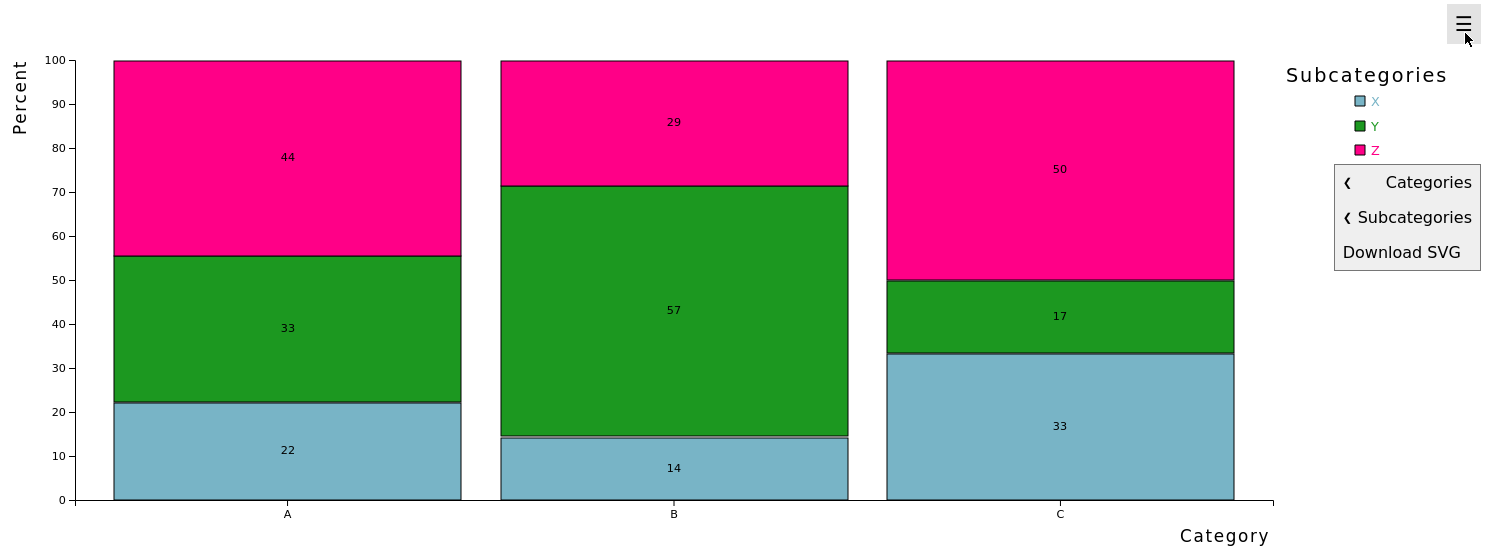
\includegraphics[keepaspectratio,width=\linewidth,height=\halfh]
{images/percent-stacked-bar-chart-window.png}
\hspace{1cm}
\label{fig:StackedBarChartWindow2}
}
\caption[Stacked Bar Chart Window Example]{%
The Stacked Bar Chart and Percent Stacked Bar Chart rendered by the source
code in Listing~\ref{list:StackedBarChartWindow}. The Tool Menu popup has
been manually displaced to not cover the legend.
\subref{fig:StackedBarChartWindow1} An ordinary Stacked Bar Chart to
compare category totals and subcategory contributions to these totals.
\subref{fig:StackedBarChartWindow2} A Percent Stacked Bar Chart to
better compare subcategory contributions to category totals.
\imgcredit{Image created by the author of this thesis using RespVis.}
}
\label{fig:StackedBarChartWindow}
\end{figure}
  







\section{Point Module}

Point charts, also commonly known as scatter charts or scatter plots,
show the relationship between two variables by plotting them as points
in a Cartesian coordinate system. Each of the two variable determines
a point's position on one of the coordinate system's two Axes, and
typically, these variables contain quantitative data. However, the
data type of the variables used to position points is not relevant, as
long as their values can be mapped to spatial dimensions via scales.
Point charts are particularly suitable for discovering potential
correlations and patterns between variables. They can also visualize
more than two variables simultaneously by encoding additional
variables via the colors, sizes, and shapes of the plotted points.
Point charts which encode an additional variable as the sizes of
points are called bubble charts.


The Point Module is located in the \code{src/lib/point/} directory of
the RespVis library and contains the implementation of Point Series,
Point Charts, and Point Chart Windows. Point Series render a
collection of \elname{<circle>} elements, whose center positions are
calculated by mapping arrays of X and Y values into the bounding boxes
of the Series' root elements via X and Y scales. The colors of points
are specified as style classes, and their radiuses can be configured,
meaning that it is also possible to create Bubble Charts with this
implementation. As with other Series, individual elements of Point
Series are rendered via a data join using an array of data objects
created through transforming the bound Series data object, and this
data join can be customized by providing custom \code{enter},
\code{update}, and \code{exit} event listeners. Point Charts are
Cartesian Charts which contain Point Series in their draw areas and two
Axes visualizing the scales used to render the Point Series.


\begin{samepage}
\lstinputlisting[%
  float=tp,
  aboveskip=\floatsep,
  belowskip=\floatsep,
  xleftmargin=0cm,              % no extra margins for floats
  xrightmargin=0cm,             % no extra margins for floats
  %
  basicstyle=\footnotesize\ttfamily,
  frame=shadowbox,
  numbers=left,
  label=list:PointChartWindow,
  caption={[Point Chart Window Example]%
Example source code to create the Point Chart Window shown in
Figure~\ref{fig:PointChartWindow}. The Point Chart Window is
configured with a bound data object initialized with the
\code{chartWindowPointData} function and rendered with the
\code{chartWindowPointRender} function. Since no special responsive
behavior is desired in this example, the default resize behavior is
attached to the Chart Window via the \code{chartWindowPointAutoResize}
function.
},
]{listings/point-chart-window.js}
\end{samepage}


Point Chart Windows are Chart Windows which contain Point Charts
nested into Layouters to handle the render process of these Charts so
that their elements can be laid out with CSS, and decorate them with a
Toolbar. Currently, the Toolbars of Point Chart Windows only contain
SVG Download Tools because only a limited number of Tools, not suited
for application on Point Charts, have been developed so far. Further
Tools that can also be applied to Point Charts, such as Zoom and
Quantitative Filter Tools, are planned for development, and once these
are available, they will be added to the default Tools attached to the
Toolbars of Point Chart Windows. Example source code to create a
scalable Point Chart Window can be found in
Listing~\ref{list:PointChartWindow}, and the resulting visualization
is shown in Figure~\ref{fig:PointChartWindow}.



\begin{figure}[tp]
\centering
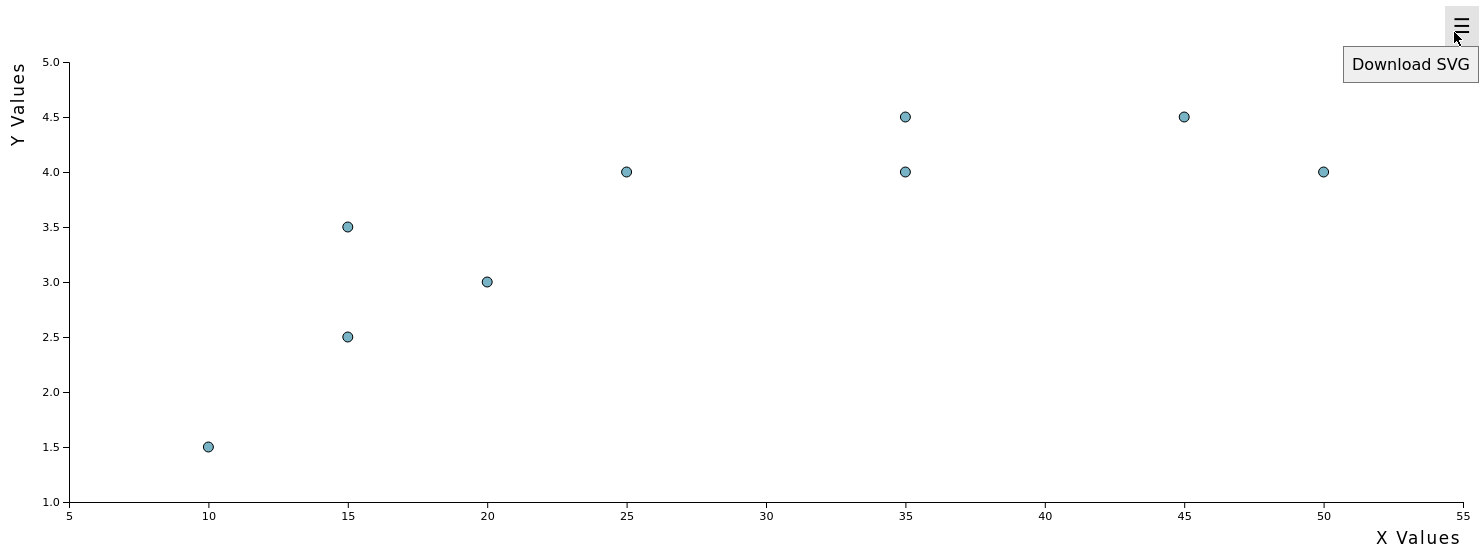
\includegraphics[keepaspectratio,width=\linewidth,height=\halfh]
{images/point-chart-window.png}
\caption[Point Chart Window Example]{%
The Point Chart Window resulting from the source code in
Listing~\ref{list:PointChartWindow}.
\imgcredit{Image created by the author of this thesis using RespVis.}
}
\label{fig:PointChartWindow}
\end{figure}
  
